\documentclass[11pt]{article}

\usepackage[utf8]{inputenc}
\usepackage[T1]{fontenc}
\usepackage{amsmath,amssymb,amsthm}
\usepackage{hyperref}
\usepackage{graphicx}
\usepackage{geometry}
\geometry{margin=2.5cm}
\usepackage{tikz}
\usepackage{pgfmath}
\usepackage{mathtools}

\newtheorem{theorem}{Theorem}

\theoremstyle{definition}
\newtheorem{definition}{Definition}[section]

\title{Trigonometry without $\pi$: a constructive approach}
\author{Daniel de Rauglaudre (alias roglo)}
\date{\today}

\begin{document}

\maketitle

\begin{abstract}
We present a construction of trigonometry where angles are not real
numbers, but pairs $(x,y)$ such that $x^2 + y^2 = 1$. Several classic
trigonometric formulas naturally emerge during this construction,
which leads to defining the division of an angle by an integer using a
convergent sequence. This construction does not require the prior
definition of the constant $\pi$, which is never used. All results are
formally proven using the Coq proof assistant.
\end{abstract}

\section{Introduction}

... to be done ...

\section{Basic Construction}

In classical trigonometry, angles are real numbers. The set \( A \) of
angles is therefore defined by

\[
A ::= \mathbb{R}
\]

\noindent Here, we set aside this definition and instead define:

\[
A ::= \{ \; (x, y) \; | \; x^2 + y^2 = 1 \; \}
\]

\noindent In other words, an angle is defined by a point on the unit
circle. This point represents the angle between the positive \( x
\)-axis and the line segment from the origin \( O \) to the point.

\

\noindent The angle \( (x, y) \) is illustrated below:

\

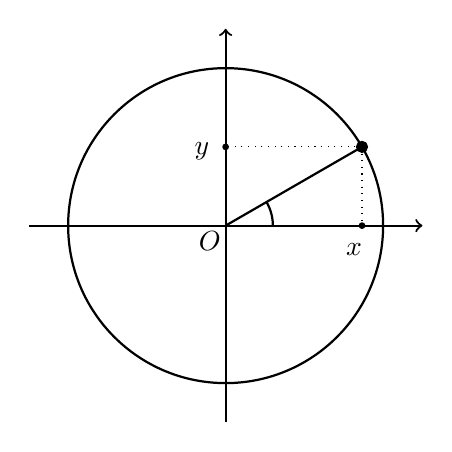
\begin{tikzpicture}
    \draw[thick] (0,0) circle(2);
    \draw[->, thick] (-2.5, 0) -- (2.5, 0);
    \draw[->, thick] (0, -2.5) -- (0, 2.5);
    \node at (-0.2,-0.2) {$O$};

    \pgfmathsetmacro{\px}{cos(30)}
    \pgfmathsetmacro{\py}{sin(30)}
    \coordinate (P) at (\px*2, \py*2);
    \draw[fill] (P) circle (2pt);
    \draw[thick] (0,0) -- (P);
    \draw[thick] (0.6,0) arc[start angle=0, end angle=30, radius=0.6];

    \draw[dotted] (P) -- (\px*2, 0);
    \draw[fill] (\px*2, 0) circle (1pt);
    \node at ({\px*2 - 0.1}, -0.3) {$x$};

    \draw[dotted] (P) -- (0, \py*2);
    \draw[fill] (0, \py*2) circle (1pt);
    \node at (-0.3, {\py*2 - 0.05}) {$y$};
\end{tikzpicture}

\

\

\noindent An angle \( \theta \) is therefore not a real number, but a triplet:

\[
\theta = (x, y, x^2 + y^2 = 1)
\]

\noindent In this setting, we define:

\[
\cos(\theta) = x \qquad \sin(\theta) = y
\]

\noindent These are our \emph{definitions} of cosine and sine. The
third component of \( \theta \) is a proof that \( x^2 + y^2 = 1
\). Note that, in traditional mathematics, proofs are not mathematical
objects. Here, we work in type theory, where proofs are themselves
objects.

\begin{theorem}
\[
\cos^2(\theta) + \sin^2(\theta) = 1
\]
\end{theorem}

\begin{proof}
By the definition of angles, this equality corresponds to the third
component of the triplet.
\end{proof}

\

\noindent In classical trigonometry, this identity requires a proof
based on the definitions of \( \cos \) and \( \sin \) as power
series. Here, no such proof is needed: the result is immediate.

\

\noindent In our approach, \( \cos \) and \( \sin \) are directly
accessed from the angle's coordinates. In classical analysis, being
defined as infinite series, they are not computable in a strict sense:
they are limits of sequences. For example, there is no algorithm that
computes \( \sin(0) \); we simply assert that the limit of the series
is zero. In that context, sine and cosine are functions in the
mathematical sense, not in the computational one.

\

\subsubsection*{Drawback}

The difficulty arises from the arithmetic of angles. In classical
trigonometry, this issue does not appear, since angles are treated as
real numbers. Any operation that is defined on the reals—addition,
subtraction, multiplication, inversion, and so on—is directly
applicable to angles.

However, when we think of angles as points on the unit circle, we can
no longer rely on the standard algebraic operations. These points, in
themselves, do not carry any inherent arithmetic structure. In order
to define such operations, we must construct them from scratch. We
begin with addition.

\section{Addition of angles}

If we have two angles $(x, y)$ and $(x', y')$, we want to define an
addition, giving a third angle $(x'', y'')$ (such that
$x''^2+y''^2=1$)

\[
(x, y) + (x', y') ::= (x'', y'')
\]

\

\noindent The solution comes from normal trigonometry. If we have two
angles $a$ and $b$, we now that

\[
cos(a+b) = cos\;a\;.\;cos\;b - sin\;a\;.\;sin\;b
\]

\[
sin(a+b) = sin\;a\;.\;cos\;b + cos\;a\;.\;sin\;b
\]

\

\noindent In our trigonometry, if we consider that the angle $(x, y)$
is named $a$, and the angle $(x', y')$ as $b$, we have

\[
(x, y) = (cos\;a, sin\;a)
\]

\[
(x, y) = (cos\;a, sin\;a)
\]

\noindent In that case, $(x'', y'')$ is $a + b$.  Applying the
classical formulas above, we can define the addition of angles as

\begin{definition}[Addition of angles]

Let $(x, y)$ and $(x', y')$ be two angles. We define a new binary
operation $\boldsymbol{+}$ by:

\[
(x, y) \boldsymbol{+} (x', y') \coloneqq (x x' - y y', x y' + y x').
\]

\end{definition}

\noindent We can also consider the points $(x, y)$ and $(x', y')$ as
the complex numbers $x+iy$ and $x'+iy'$ and define addition as the
product of these complex numbers, giving the same result, since it is
well known that multiplication of complex numbers is addition or their
angles.

...

\section{Conclusion}

... to be done ...

\paragraph{Code source :}
\url{https://github.com/roglo/coq_sensitivity/tree/master/trigo_without_pi}

\end{document}
